%\vspace{-0.11in}
\chapter{System Overview}\label{overview}
\section{Chain of Events in an IoT System}
Figure~\ref{chainreaction} illustrates a high level view of the chain of events in an IoT system.
In brief, sensors sense the physical world and convert them into events in the cyber world;
these events, in turn, are passed onto apps that subscribe to such events.
Upon processing the cyber events these apps may
output commands to actuators, which
then trigger new physical or cyber events.
Apps may also directly generate new cyber events.
Therefore, a single event could lead to a large sequence of subsequent cyber/physical events.
%which could translate to a large state space to check.

\begin{figure}[tb]
\begin{center}
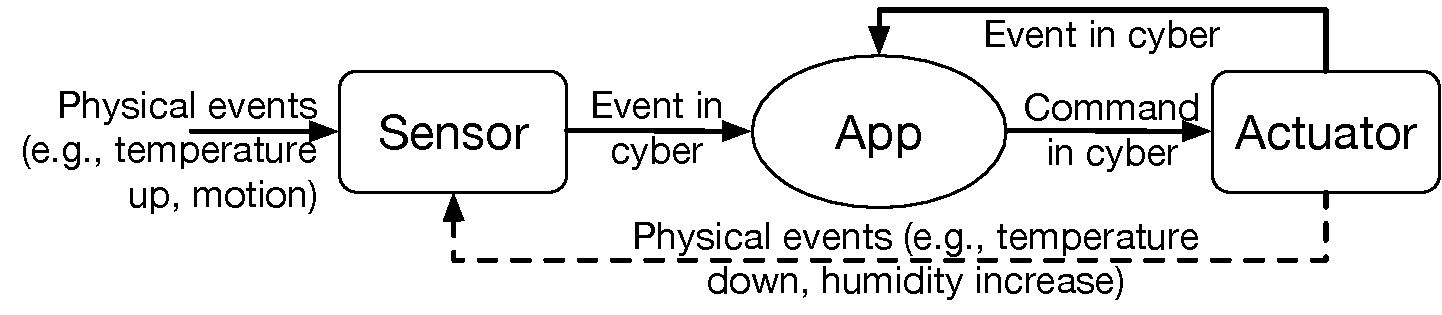
\includegraphics[width=3.5in]{chainreaction}
%\vspace{-0.17in}
\caption{Chain of events in an IoT system.}
\label{chainreaction}
\end{center}
%\vspace{-0.23in}
\end{figure}

%Moreover, state change events of actuators may trigger some apps \thomas{Do we need to talk about the permutation of input events here}. Therefore, with a single physical event, there may be many events generated in the cyber world. That is, the state space may get exponentially exploded with just a small amount of input physical events.

\section{Overall Architecture}
Figure~\ref{iSanitizerArchitecture} depicts the architecture of our system \sys.
It consists of five modules viz.,
\textit{App Dependency Analyzer}, \textit{Translator}, \textit{Configuration Extractor}, \textit{Model Generator}, and \textit{Output Analyzer}.
In designing \sys, we tackle two main challenges:
(i) alleviating the state space explosion with model checking~\cite{Clarke2012} for our context, and
(ii) the translation of smart apps' source code to Promela (to facilitate model checking).
We address the first problem partially in the \textit{App Dependency Analyzer}
and partially in the \textit{Model Generator}.
The second problem is handled partially in the \textit{Translator}
and partially in the \textit{Model Generator}.

\begin{figure}[tb]
\begin{center}
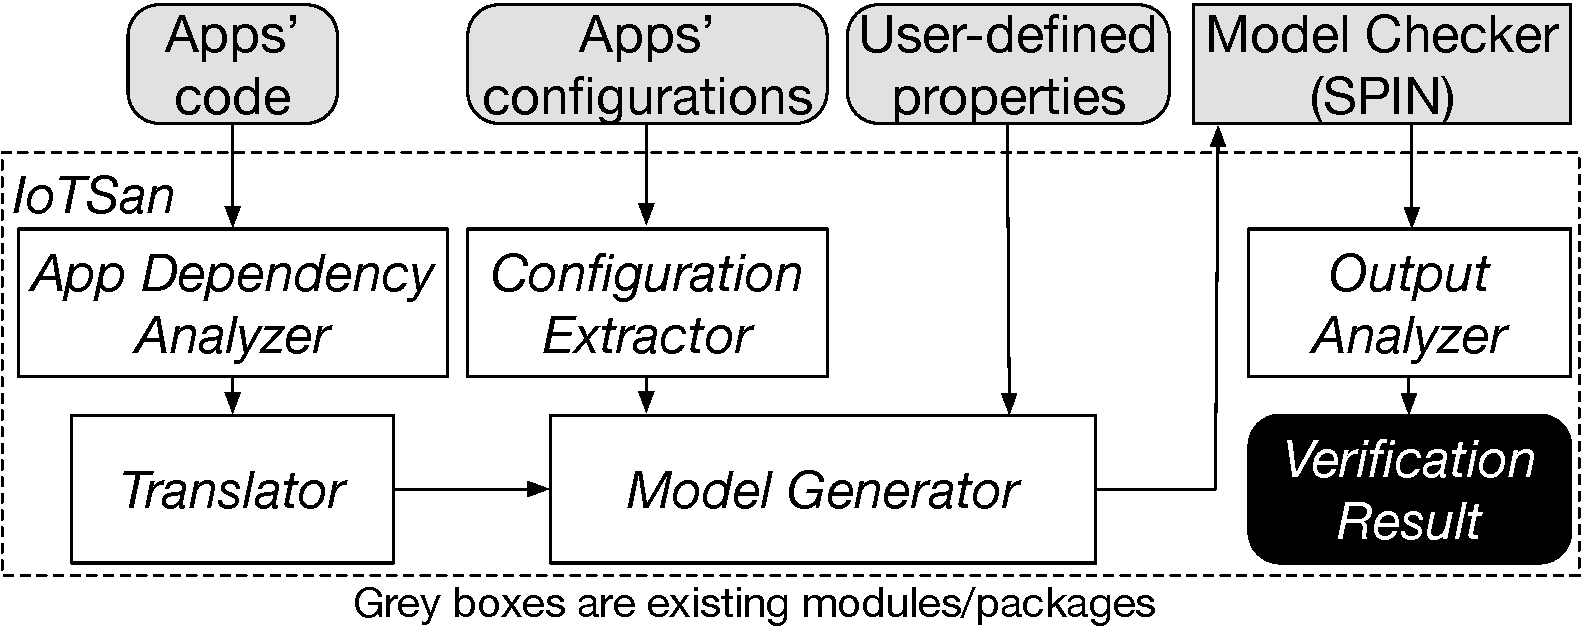
\includegraphics[width=3.1in]{iSanitizerArchitecture}
%\vspace{-0.1in}
\caption{\sys architecture overview.}
\label{iSanitizerArchitecture}
\end{center}
%\vspace{-0.25in}
\end{figure}

\textbf{\em App Dependency Analyzer} (\S~\ref{sec:depedency}):
This module constructs dependency graphs to capture
interactions between {\color{black}event handlers of different apps
and identifies handlers that must be jointly analyzed by the model checker.
This precludes the unnecessary analysis of unrelated event handlers.}
%Then, we verify only the apps in the same dependent set together while excluding other unrelated apps.

\textbf{\em Translator} (\S~\ref{sec:translator}):
%To the best of our knowledge, there are no model checking systems that readily verify Groovy programs.
We build a translator within \sys, that automatically converts Groovy programs into Promela.
In doing so, we address the following challenges:
\begin{itemize}
\item {\em Implicit Types}. In Groovy programs, data types of variables and return types of functions are not
explicitly declared. To solve this problem, we design an algorithm to infer data types of variables and return types of functions.
%\krish{People frown at heuristics. Can we say something else - or at least why this is good ?} \thomas{I have changed it to \textit{context-based}}
\item {\em Built-in Utilities}. Groovy has many built-in utilities,
\textit{e.g.}, \texttt{find}, \texttt{findAll}, \texttt{each}, \texttt{collect},
\texttt{first}, $+$ on list types, and \texttt{map}.
We manually analyzed the behavior of each utility and translated them into corresponding code in Promela.
%\krish{I don't think we should say "we have to". Did we do this ? Was this manual? This part is vague otherwise.} \thomas{We manually analyze the behaviors but the translation process is automatic.}
\end{itemize}
%The \textit{Translator} module outputs the Promela code of apps' event handlers.

\textbf{\em Configuration Extractor} (\S~\ref{sec:extractor}):
IoT platforms often provide a companion mobile app and/or
web-based app to manage/configure the installed smart apps and devices of an IoT system.
This module automatically extracts the system's configurations from the manager app.
%It also gets a list of desired properties from the user.

\textbf{\em Model Generator} (\S~\ref{sec:model}):
This module takes the Promela code of event handlers,
the configuration of the IoT system, and safety properties (both pre-defined and user-defined) as inputs,
and creates the Promela model of the system.
We use sequential design to model the IoT system instead of concurrent design.
This significantly reduces the problem size by eliminating
unnecessary interleaving that is unlikely to yield useful assessment of unsafe behaviors.
The generated model is checked by \spin for possible property violations.

\textbf{\em Output Analyzer} (\S~\ref{outputanalyzer}):
This module analyzes the verification logs and attributes safety violations to potentially malicious apps,
bad designs or misconfiguration.
Based on the result, it provides the user, a suggestion to either remove a bad app(s) or change an app(s)'s
configuration.

%{\color{violet}Table~\ref{table:comparison} shows the comparison of \sys and related work (more details in \S~\ref{sec:related}).}

\begin{table}[t]
\scriptsize
\ssp
%\vspace{-0.12in}
\caption{Comparison of \sys and related work.}
%\vspace{-0.12in}
\label{table:comparison}
\centering
\begin{tabular}{| p{5cm} | c | c | c | c |}
\hline
\textbf{Feature} & \textbf{SIFT \cite{Liang:2015:SBI:2737095.2737115}} & \textbf{DeLorean \cite{190480}} & \textbf{Soteria \cite{215955}} & \textbf{\sys}\\
\hline
Detects physical safety violations & \Checkmark & \Checkmark & \Checkmark & \Checkmark\\
\hline
Detects information leakage &  &  &  &  \Checkmark\\
\hline
Detects violations due to communication/device failures &  &  &  &  \Checkmark\\
\hline
Detects violations due to misconfiguration problems &  &  &  &  \Checkmark\\
\hline
Handles complex code beyond IFTTT rules &  & \Checkmark & \Checkmark & \Checkmark\\
\hline
Performs violation attribution &  &  &  &  \Checkmark\\
\hline
%Targets legacy apps & \Checkmark & \Checkmark & \Checkmark &  & \Checkmark\\
%\hline
Accounts for app interactions & \Checkmark &  & \Checkmark & \Checkmark\\
\hline
%\textbf{No need for app patches} &  &  &  &  & \Checkmark\\
%\hline
%Platform compliant &  & \Checkmark &  & \Checkmark & \Checkmark\\
%\hline
\end{tabular}
%\vspace{-0.21in}
\end{table}

\begin{comment}
\begin{table}[t]
\scriptsize
%\vspace{-0.12in}
\caption{Comparison of \sys and related work.}
%\vspace{-0.12in}
\label{table:comparison}
\centering
\begin{tabular}{| p{1.9cm} | p{1.05cm} | p{1.12cm} | p{1.15cm} | p{0.45cm} | p{0.6cm} |}
\hline
\textbf{Feature} & \textbf{SIFT \cite{Liang:2015:SBI:2737095.2737115}} & \textbf{DeLorean \cite{190480}} & \textbf{Soteria \cite{215955}} & \textbf{SIFT \cite{Liang:2015:SBI:2737095.2737115}} & \textbf{\sys}\\
\hline
\textbf{Detects physical safety violations} & \Checkmark & \Checkmark & \Checkmark & \Checkmark & \Checkmark\\
\hline
\textbf{Detects information leakage} &  &  &  &  & \Checkmark\\
\hline
\textbf{Detects violations due to communication failures} &  &  &  &  & \Checkmark\\
\hline
\textbf{Detects violations due to misconfiguration problems} &  &  &  &  & \Checkmark\\
\hline
\textbf{Handles complex code beyond IFTTT rules} &  & \Checkmark & \Checkmark & \Checkmark & \Checkmark\\
\hline
\textbf{Performs violation attribution} &  &  &  &  & \Checkmark\\
\hline
%Targets legacy apps & \Checkmark & \Checkmark & \Checkmark &  & \Checkmark\\
%\hline
\textbf{Accounts for app interactions} &  &  &  & \Checkmark & \Checkmark\\
\hline
%\textbf{No need for app patches} &  &  &  &  & \Checkmark\\
%\hline
%Platform compliant &  & \Checkmark &  & \Checkmark & \Checkmark\\
%\hline
\end{tabular}
%\vspace{-0.1in}
\end{table}
\end{comment}

%\subsection{Overall Architecture}
%Figure \ref{iSanitizerArchitecture} shows the overall architecture of our proposed system - \sys. The input of our system, which comprises of smart apps' source code and their configurations from users, goes into the \textit{App Dependency Analysis}, whose output are sets of dependent apps. The apps in each dependent set are fed into the \textit{Translator}. The result of the \textit{Translator} is in form of an intermediate representation (IR), \textit{e.g.}, Jimple. The \textit{Model Generator} takes apps' IR and configurations as inputs, and then creates a model in the target language of the model checker. In this paper, we use Spin for the model checker. Thus, the result of \textit{Model Generator} is  a Promela model, which is then verified by the Spin model checker. The verification result is checked by the \textit{Output Analyzer}. If detecting any violation, \textit{Output Analyzer} will attribute it to either bad app or bad configuration. The final result given to users is either (ii) no violation or (ii) suggestion to either remove some bad apps or change apps' configuration.

% \textbf{User Inputs}: \textcolor{black}{Upon installation, a user needs
% to configure a smart
% app. Poor configurations
% may cause the IoT system to transition to unsafe physical states.
% There are many common causes for such configurations. These are: (i) the app's description is not clear or misleading, (ii) there are too many configuration options, and (iii) normal users often do not have good domain knowledge to clearly understand the behaviors of smart devices and smart apps. To exemplify these issues, consider the following example. Figure \ref{inputexample} shows the input info that the app \textit{Virtual Thermostat} needs
% from a user. First, the description of the app is vague and states ``Control a space heater or window air conditioner (AC) in conjunction with any temperature sensor, like a SmartSense Multi."  \textit{Virtual Thermostat} asks users to configure a
% temperature measurement sensor (lines 2-5), the {\color{black} power} outlets into
% which the heater and the AC are plugged into (lines 6-9), a desired temperature (lines 10-12),
% etc.
% This seems to suggest that the app controls {\em both} the heater and the AC
% to maintain the desired temperature; however, it only expects one type of device.
% Second, since power outlets are used to control many type of devices (\textit{e.g.}, smart bulb, TV, AC, and heater), the SmartThings displays (exports) all of the outlets (capability.switch) in the IoT system to the user; in other words
% there are too many configuration options provided to the user.
% }

% %\krish{Did we discuss the user study before at all, it comes abruptly -- and we don't say why we do this. Should we say this somewhere earlier?}
% Finally, to showcase (iii)
% we conduct a user study (more details in \S~\ref{sec:eval})
% where we asked 7 student volunteers to configure various apps as they deemed fit.
% In this case, 5 out of 7 student volunteers configure the app to control both the AC and the heater (which it is not equipped to do). This caused the following. \textcolor{black}{When the temperature is higher than a predefined threshold, the \textit{Virtual Thermostat} turned on both the configured outlets, \textit{i.e.}, both the heater and the AC are turned on!
% As evident, this violates the following two
% commonsense properties: (i) a heater is turned on when temperature is {\color{black}above a predefined threshold}, and (iii) an AC and a heater are both turned on.}
% %\textcolor{red}{Note that we may have problem only when an AC and a heater in the same room/house are both turned on, \textit{i.e.}, this may not be a violation if the two devices are at different locations; and we let the user decide which properties their IoT system should satisfy.}

\section{Our Work in Perspective} \sys can be envisioned as a service 
that jointly considers the apps, devices and their configurations of an IoT system, and checks whether a set of a priori defined properties hold. In addition to detecting safety violations of the physical space, it also detects information leakage. {\color{black}
Finally, it also determines if communication/device failures can cause unsafe states and detects violations due to misconfiguration problems}. In Table~\ref{table:comparison} we show the features that
\sys offers compared to the most related recent systems. A discussion of related work is deferred to \S~\ref{sec:related}.
